\chapter{End of chapter exercise solutions}
\label{eoceSolutions}

\eocesolch{Data collection}

%%%%%%%%%%%%%%%%%%%%%%%%%%%%%

\begin{multicols}{2}

% 1
\eocesol{(a) Treatment: $10/43 = 0.23 \rightarrow 23\%$. Control: $2/46 = 0.04 \rightarrow 4\%$. (b) There is a 19\% difference between the pain reduction rates in the two groups. At first glance, it appears patients in the treatment group are more likely to experience pain reduction from the acupuncture treatment. (c) Answers may vary but should be sensible. Two possible answers: $^1$Though the groups' difference is big, I'm skeptical the results show a real difference and think this might be due to chance. $^2$The difference in these rates looks pretty big, so I suspect acupuncture is having a positive impact on pain.}

% 3
\eocesol{(a-i) 143,196 eligible study subjects born in Southern California between 1989 and 1993. (a-ii) Measurements of carbon monoxide, nitrogen dioxide, ozone, and particulate matter less than 10$\mu g/m^3$ (PM$_{10}$) collected at air-quality-monitoring stations as well as length of gestation. These are continuous numerical variables. (a-iii) The research question: ``Is there an association between air pollution exposure and preterm births?" (b-i) 600 adult patients aged 18-69 years diagnosed and currently treated for asthma. (b-ii) The variables were whether or not the patient practiced the Buteyko method (categorical) and measures of quality of life, activity, asthma symptoms and medication reduction of the patients (categorical, ordinal). It may also be reasonable to treat the ratings on a scale of 1 to 10 as discrete numerical variables. (b-iii) The research question: ``Do asthmatic patients who practice the Buteyko method experience improvement in their condition?"}

% 5
\eocesol{(a) $50 \times 3 = 150$. (b) Four continuous numerical variables: sepal length, sepal width, petal length, and petal width. (c) One categorical variable, species, with three levels: \emph{setosa}, \emph{versicolor}, and \emph{virginica}.}

%\Comment{these two need to rewritten to not reference something far back}
% Unclear what this is referring to (what is "these" and "something"?)

% 7
\eocesol{(a) Population of interest: all births in Southern California. Sample: 143,196 births between 1989 and 1993 in Southern California. If births in this time span can be considered to be representative of all births, then the results are generalizable to the population of Southern California. However, since the study is observational, the findings do not imply causal relationships. (b) Population: all 18-69 year olds diagnosed and currently treated for asthma. Sample: 600 adult patients aged 18-69 years diagnosed and currently treated for asthma. Since the sample consists of voluntary patients, the results cannot necessarily be generalized to the population at large. However, since the study is an experiment, the findings can be used to establish causal relationships.}

% 9
\eocesol{(a) Explanatory: number of study hours per week. Response: GPA. 
(b) There is a slight positive relationship between the two variables. One respondent reported a GPA above 4.0, which is a data error. There are also a few respondents who reported unusually high study hours (60 and 70 hours/week). The variability in GPA also appears to be larger for students who study less than those who study more. Since the data become sparse as the number of study hours increases, it is somewhat difficult to evaluate the strength of the relationship and also the variability across different numbers of study hours.
(c) Observational.
(d) Since this is an observational study, a causal relationship is not implied.}

% 11
\eocesol{(a) Observational.
(b) The professor suspects students in a given section may have similar feelings about the course. To ensure each section is reasonably represented, she may choose to randomly select a fixed number of students, say 10, from each section for a total sample size of 40 students. Since a random sample of fixed size was taken within each section in this scenario, this represents stratified sampling.}

% 13
\eocesol{Sampling from the phone book would miss unlisted phone numbers, so this would result in bias. People who do not have their numbers listed may share certain characteristics, e.g. consider that cell phones are not listed in phone books, so a sample from the phone book would not necessarily be a representative of the population.}

% 15
\eocesol{The estimate will be biased, and it will tend to overestimate the true family size. For example, suppose we had just two families: the first with 2 parents and 5 children, and the second with 2 parents and 1 child. Then if we draw one of the six children at random, 5 times out of 6 we would sample the larger family}

% 17
\eocesol{(a) No, this is an observational study.
(b) This statement is not justified; it implies a causal association between sleep disorders and bullying. However, this was an observational study. A better conclusion would be ``School children identified as bullies are more likely to suffer from sleep disorders than non-bullies.''}

% 19
\eocesol{(a) Experiment, as the treatment was assigned to each patient.
(b)~Response: Duration of the cold. Explanatory: Treatment, with 4 levels: \emph{placebo}, \emph{1g}, \emph{3g}, \emph{3g with additives}.
(c)~Patients were blinded.
(d)~Double-blind with respect to the researchers evaluating the patients, but the nurses who briefly interacted with patients during the distribution of the medication were not blinded. We could say the study was partly double-blind.
(e)~No. The patients were randomly assigned to treatment groups and were blinded, so we would expect about an equal number of patients in each group to not adhere to the treatment.}

% 21
\eocesol{(a) Experiment.
(b)~Treatment is exercise twice a week. Control is no exercise. 
(c)~Yes, the blocking variable is age.
(d)~No.
(e)~This is an experiment, so a causal conclusion is reasonable. Since the sample is random, the conclusion can be generalized to the population at large. However, we must consider that a placebo effect is possible. 
(f)~Yes. Randomly sampled people should not be required to participate in a clinical trial, and there are also ethical concerns about the plan to instruct one group not to participate in a healthy behavior, which in this case is exercise.}

\end{multicols}
\eocesolch{Summarizing data}

%%%%%%%%%%%%%%%%%%%%%%%%%%%%%
\begin{multicols}{2}
% 1
\eocesol{(a) Positive association: mammals with longer gestation periods tend to live longer as well.
(b)~Association would still be positive.
(c)~No, they are not independent. See part~(a).}

% 3
\eocesol{(a) 1/linear and 3/nonlinear.
(b)~4/some curvature (nonlinearity) may be present on the right side. ``Linear'' would also be acceptable for the type of relationship for plot~4.
(c)~2.}

% 5
\eocesol{(a)~Decrease: the new score is smaller than the mean of the 24 previous scores.
(b)~Calculate a weighted mean. Use a weight of 24 for the old mean and 1 for the new mean: $(24\times 74 + 1\times64)/(24+1) = 73.6$. There are other ways to solve this exercise that do not use a weighted mean.
(c)~The new score is more than 1 standard deviation away from the previous mean, so increase.}

% 7
\eocesol{Both distributions are right skewed and bimodal with modes at 10 and 20 cigarettes; note that people may be rounding their answers to half a pack or a whole pack. The median of each distribution is between 10 and 15 cigarettes. The middle 50\% of the data (the IQR) appears to be spread equally in each group and have a width of about 10 to 15. There are potential outliers above 40 cigarettes per day. It appears that respondents who smoke only a few cigarettes (0 to 5) smoke more on the weekdays than on weekends.}

% 9
\eocesol{(a) $\bar{x}_{amtWeekends} = 20$, $\bar{x}_{amtWeekdays} = 16$.
(b) $s_{amtWeekends} = 0$, $s_{amtWeekdays} = 4.18$. In this very small sample, higher on weekdays.}

% 11
\eocesol{(a) Both distributions have the same median and IQR.
(b) Second distribution has a higher median and higher IQR.
(c) Second distribution has higher median. IQRs are equal.
(d) Second distribution has higher median and larger IQR.}


% 13
\eocesol{\vspace{-4mm}\\\includegraphics[width = 0.4\textwidth]{ch_data_collection/figures/eoce/statsFinalScores/statsFinalScores_box}}

% 15
\eocesol{Descriptions will vary a little. (a)~2. Unimodal, symmetric, centered at 60, standard deviation of roughly 3.
(b)~3. Symmetric and approximately evenly distributed from 0 to 100.
(c)~1. Right skewed, unimodal, centered at about 1.5, with most observations falling between 0 and 3. A very small fraction of observations exceed a value of 5.}

% 17
\eocesol{The histogram shows that the distribution is bimodal, which is not apparent in the box plot. The box plot makes it easy to identify more precise values of observations outside of the whiskers.}

% 19
\eocesol{(a) The median is better; the mean is substantially affected by the two extreme observations.
(b) The IQR is better; the standard deviation, like the mean, is substantially affected by the two high salaries.}

% 21
\eocesol{The distribution is unimodal and symmetric with a mean of about 25 minutes and a standard deviation of about 5 minutes. There does not appear to be any counties with unusually high or low mean travel times. Since the distribution is already unimodal and symmetric, a log transformation is not necessary.}

% 23
\eocesol{Answers will vary. There are pockets of longer travel time around DC, Southeastern NY, Chicago, Minneapolis, Los Angeles, and many other big cities. There is also a large section of shorter average commute times that overlap with farmland in the Midwest. Many farmers' homes are adjacent to their farmland, so their commute would be 0 minutes, which may explain why the average commute time for these counties is relatively low.}

% 25
\eocesol{(a)~We see the order of the categories and the relative frequencies in the bar plot.
(b)~There are no features that are apparent in the pie chart but not in the bar plot.
(c)~We usually prefer to use a bar plot as we can also see the relative frequencies of the categories in this graph.}


% 27
\eocesol{(a) False. Instead of comparing counts, we should compare percentages.
(b)~True.
(c) False. We cannot infer a causal relationship from an association in an observational study. However, we can say the drug a person is on affects his risk in this case, as he chose that drug and his choice may be associated with other variables, which is why part~(b) is true. The difference in these statements is subtle but important.
(d)~True.}

% 29
\eocesol{(a) Proportion who had heart attack: $\frac{7,979}{227,571} \approx 0.035$
(b) Expected number of cardiovascular problems in the rosiglitazone group if having cardiovascular problems and treatment were independent can be calculated as the number of patients in that group multiplied by the overall rate of cardiovascular problems in the study: $\text{67,593} \times \frac{\text{7,979}}{\text{227,571}} \approx 2370$.
(c-i) $H_0$: Independence model. The treatment and cardiovascular problems are independent. They have no relationship, and the difference in incidence rates between the rosiglitazone and pioglitazone groups is due to chance.
$H_A$: Alternate model. The treatment and cardiovascular problems are not independent. The difference in the incidence rates between the rosiglitazone and pioglitazone groups is not due to chance, and rosiglitazone is associated with an increased risk of serious cardiovascular problems.
(c-ii) A higher number of patients with cardiovascular problems in the rosiglitazone group than expected under the assumption of independence would provide support for the alternative hypothesis. This would suggest that rosiglitazone increases the risk of such problems.
(c-iii) In the actual study, we observed 2,593 cardiovascular events in the rosiglitazone group. In the 1,000 simulations under the independence model, we observed somewhat less than 2,593 in all simulations, which suggests that the actual results did not come from the independence model. That is, the analysis provides strong evidence that the variables are not independent, and we reject the independence model in favor of the alternative. The study's results provide strong evidence that rosiglitazone is associated with an increased risk of cardiovascular problems.}

\end{multicols}




\eocesolch{Probability}

\begin{multicols}{2}

% 1
\eocesol{(a)~False. These are independent trials.
(b)~False. There are red face cards.
(c)~True. A card cannot be both a face card and an ace.}

% 3
\eocesol{(a) 10 tosses. Fewer tosses mean more variability in the sample fraction of heads, meaning there's a better chance of getting at least 60\% heads.
(b) 100 tosses. More flips means the observed proportion of heads would often be closer to the average, 0.50, and therefore also above 0.40.
(c) 100 tosses. With more flips, the observed proportion of heads would often be closer to the average, 0.50.
(d) 10 tosses. Fewer flips would increase variability in the fraction of tosses that are heads.}

% 5

\eocesol{(a)~$0.5^{10}$ = 0.00098.
(b)~$0.5^{10}$ = 0.00098.
(c)~$P$(at least one tails) = $1 - P$(no tails) = $1 - (0.5^{10}) \approx 1 - 0.001 = 0.999$.}

% 7
\eocesol{(a)~No, there are voters who are both politically Independent and also swing voters.
(b)~Venn diagram below: \\
\includegraphics[width=0.2\textwidth]{ch_summarizing_data/figures/eoce/indepSwing/indepSwing} \\
(c)~24\%.
(d)~Add up the corresponding disjoint sections in the Venn diagram: $0.24 + 0.11 + 0.12 = 0.47$. Alternatively, use the General Addition Rule: $0.35 + 0.23 - 0.11 = 0.47$.
(e)~$1 - 0.47 = 0.53$.
(f)~$P$(Independent) $\times$ $P$(swing) = $0.35\times0.23 = 0.08$, which does not equal P(Independent and swing) = 0.11, so the events are dependent. If you stated that this difference might be due to sampling variability in the survey, that answer would also be reasonable (we'll dive into this topic more in later chapters).}

% 9
\eocesol{(a) If the class is not graded on a curve, they are independent. If graded on a curve, then neither independent nor disjoint (unless the instructor will only give one A, which is a situation we will ignore in parts~(b) and~(c)).
(b) They are probably not independent: if you study together, your study habits would be related, which suggests your course performances are also related.
(c) No. See the answer to part~(a) when the course is not graded on a curve. More generally: if two things are unrelated (independent), then one occurring does not preclude the other from occurring.}

% 11
\eocesol{(a)~$0.16 + 0.09 = 0.25$.
(b)~$0.17 + 0.09 = 0.26$.
(c)~Assuming that the education level of the husband and wife are independent: $0.25 \times 0.26 = 0.065$. You might also notice we actually made a second assumption: that the decision to get married is unrelated to education level.
(d)~The husband/wife independence assumption is probably not reasonable, because people often marry another person with a comparable level of education. We will leave it to you to think about whether the second assumption noted in part~(c) is reasoanble.}

% 13
\eocesol{(a)~Invalid. Sum is greater than 1.
(b)~Valid. Probabilities are between 0 and 1, and they sum to 1. In this class, every student gets a C.
(c)~Invalid. Sum is less than 1.
(d)~Invalid. There is a negative probability.
(e)~Valid. Probabilities are between 0 and 1, and they sum to 1.
(f)~Invalid. There is a negative probability.}

% 15
\eocesol{(a)~No, but we could if A and B are independent.
(b-i)~0.21.
(b-ii)~$0.3+0.7-0.21=0.79$.
(b-iii)~Same as $P(A)$: 0.3. 
(c)~No, because 0.1 $\ne$ 0.21, where 0.21 was the value computed under independence from part~(a).
(d)~$P($A$|$B$) = 0.1 / 0.7 = 0.143$.}

% 17
\eocesol{(a)~$0.60 + 0.20 - 0.18 = 0.62$.
(b)~$0.18/0.20 = 0.90$.
(c)~$0.11/0.33 \approx 0.33$.
(d)~No, otherwise the final answers of parts (b) and (c) would have been equal.
(e)~$0.06/0.34 \approx 0.18$.}

% 19
\eocesol{(a) $162/248 = 0.65$.
(b) $181/252 = 0.72$
(c) Under the assumption of a dating choices being independent of hamburger preference, which on the surface seems reasonable: $0.65 \times 0.72 = 0.468$.
(d) $(252 + 6 - 1)/500 = 0.514$}

% 21
\eocesol{(a) 0.3.
(b) 0.3.
(c) 0.3.
(d) $0.3\times0.3=0.09$.
(e) Yes, the population that is being sampled from is identical in each draw.}

% 23
\eocesol{(a) 2/9.
(b) $3/9=1/3$.
(c) $(3/10)\times(2/9) \approx 0.067$.
(d) No. In this small population of marbles, removing one marble meaningfully changes the probability of what might be drawn next.}

% 25
\eocesol{For 1 leggings (L) and 2 jeans (J), there are three possible orderings: LJJ, JLJ, and JJL. The probability for LJJ is $(5/24)\times(7/23)\times(6/22) = 0.0173$. The other two orderings have the same probability, and these three possible orderings are disjoint events. Final answer: 0.0519.}


% 27
\eocesol{(a) The tree diagram:
\begin{center}
\includegraphics[width=0.48\textwidth]{ch_probability/figures/eoce/tree/tree_boxPlot}
\end{center}
(b) $P(\text{\scriptsize can~construct} | \text{\scriptsize pass}) = \frac{P(\text{\scriptsize can~construct~and~pass})}{P(\text{\scriptsize pass})} = \frac{0.8  \times 0.86}{0.8 \times 0.86\  +\  0.2 \times 0.65} = \frac{0.688}{0.818} \approx 0.84$.}


% 29
\eocesol{First draw a tree diagram:
\begin{center}
\includegraphics[width=0.45\textwidth]{ch_probability/figures/eoce/tree/tree_swazilandHIV}
\end{center}
Then compute the probability: $P(HIV | +) = \frac{P(HIV~and~+)}{P(+)} = \frac{0.259 \times 0.997}{0.259 \times 0.997 + 0.741 \times 0.074}= \frac{0.2582}{0.3131} = 0.8247$.}


% 31
\eocesol{A tree diagram of the situation:
\begin{center}
\includegraphics[width=0.48\textwidth]{ch_probability/figures/eoce/tree/tree_lupus}
\end{center}
$P(\text{lupus} | \text{positive}) = \frac{P(\text{\text{lupus~and~positive}})}{P(\text{positive})} = \frac{0.0196}{0.0196 + 0.2548} = 0.0714$. Even when a patient tests positive for lupus, there is only a 7.14\% chance that he actually has lupus. While House is not exactly right -- it is possible that the patient has lupus -- his implied skepticism is warranted.}


% 33
\eocesol{(a)~$\stackrel{Anna}{1/5}\times\stackrel{Ben}{1/4}\times\stackrel{Carl}{1/3}\times\stackrel{Damian}{1/2}\times\stackrel{Eddy}{1/1} = 1/5!=1/120$.
(b)~Since the probabilities must add to 1, there must be $5!=120$ possible orderings.
(c)~$8!=\text{40,320}$.}

% 35
\eocesol{(a) Yes. The conditions are satisfied: independence, fixed number of trials, either success or failure for each trial, and probability of success being constant across trials.
(b) 0.200.
(c) 0.200.
(d) $0.0024 + 0.0284 + 0.1323 = 0.1631$.
(e) $1-0.0024 = 0.9976$.}

% 37
\eocesol{(a)~If 13\% of the students smoke, then we expect about $0.13 \times 100 = 13$ to smoke in the sample.
(b)~No, since this is not a random sample of students, so it may not be representative with respect to smoking behavior.}

\end{multicols}

% 39
\eocesol{(a)~The table below summarizes the probability model:
\begin{center}\tiny
\begin{tabular} { l | l | l | l | l | l}
Event 	& X		& P(X)										& X $\cdot$ P(X) 	& $(X - E(X))^2$	& $(X - E(X))^2 \cdot P(X)$ \\
\hline
3 hearts	& 50		& $\frac{13}{52} \times \frac{12}{51} \times \frac{11}{50} = 0.0129$	& 0.65		& $(50 - 3.59)^2 = 2154.1 $	& $2154.1 \times 0.0129 = 27.9$ 	 \\
3 blacks	& 25		& $\frac{26}{52} \times \frac{25}{51} \times \frac{24}{50} = 0.1176$	& 2.94		& $(25 - 3.59)^2 = 458.5 $	& $458.5 \times 0.1176 = 53.9$  \\
Else		& 0		& $1 - (0.0129 + 0.1176) = 0.8695$					& 0 			& $(0 - 3.59)^2 = 12.9 $	& $12.9 \times 0.8695 = 11.2$ \\
\hline
		&		&											& E(X) = \$3.59 & 						& $V(X) = 93.0 $ \\
\multicolumn{5}{l |}{}  																				& $SD(X) = \sqrt{V(X)} = 9.64$
\end{tabular}
\end{center}
(b)~$E(X - 5) = E(X) - 5 = 3.59 - 5 = -\$1.41$. The standard deviation is the same as the standard deviation of $X$: \$9.64.
(c)~No. The expected earnings is negative, so on average you would lose money playing the game.}

\textPE{\pagebreak}

\begin{multicols}{2}

% 41
\eocesol{\begin{center}\scriptsize
\renewcommand{\arraystretch}{1.5}
\begin{tabular} {l | l | l | l}
Event 		& $X$ 	& $P(X)$ 			& $X \cdot P(X)$	  \\
\hline
Boom		& 0.18	& $\frac{1}{3}$ 		& $0.18 \times \frac{1}{3} = 0.06$ 	  \\
Normal		& 0.09	& $\frac{1}{3}$ 		& $0.09 \times \frac{1}{3} = 0.03$  \\
Recession	& -0.12	& $\frac{1}{3}$		& $-0.12 \times \frac{1}{3} = -0.04$  \\
\hline
&&& $E(X) = 0.05$ 
\end{tabular}
\end{center}
The expected return is a 5\% increase in value for a single year.}


% 43
\eocesol{(a)~Expected: -\$0.16. Variance: 8.95. SD:~\$2.99.
(b)~Expected: -\$0.16. SD:~\$1.73.
(c)~Expected values are the same, but the SDs differ. The SD from the game with tripled winnings/losses is larger, since the three independent games might go in different directions (e.g. could win one game and lose two games).  So the three independent games is lower risk, but in this context it just means we are likely to lose a more stable amount since the expected value is still negative.}

% 45
\eocesol{A fair game has an expected value of zero. From the friend's perspective: $-\$5 \times 0.54 + x \times 0.46 = 0$. Solving for $x$: \$5.87. You would bet \$5.87 for the Padres to make the game fair.}

% 47
\eocesol{(a)~Expected: \$3.90. SD: \$0.34.
(b)~Expected: \$27.30. SD: \$0.89. If you computed part~(b) using part~(a), you should have obtained an SD of \$0.90.}

% 49
\eocesol{Approximate answers are OK. Answers are only estimates based on the sample. (a)~$(29+32)/144 = 0.42$.
(b)~$21/144 = 0.15$.
(c)~$(26+12+15)/144 = 0.37$.}

\end{multicols}






\eocesolch{Distributions of random variables}

\begin{multicols}{2}

% 1
\eocesol{(a)~8.85\%.
(b)~6.94\%.
(c)~58.86\%.
(d)~4.56\%. \\
\includegraphics[width=0.23\textwidth]{ch_distributions/figures/eoce/z/zltNeg}
\includegraphics[width=0.23\textwidth]{ch_distributions/figures/eoce/z/zgtPos}
\includegraphics[width=0.23\textwidth]{ch_distributions/figures/eoce/z/zBet}
\includegraphics[width=0.23\textwidth]{ch_distributions/figures/eoce/z/zgtAbs}}

% 3
\eocesol{(a)~Verbal: $N(\mu = 462, \sigma = 119)$, Quant: $N(\mu = 584, \sigma = 151)$.
(b)~$Z_{VR} = 1.33$, $Z_{QR} = 0.57$. \\
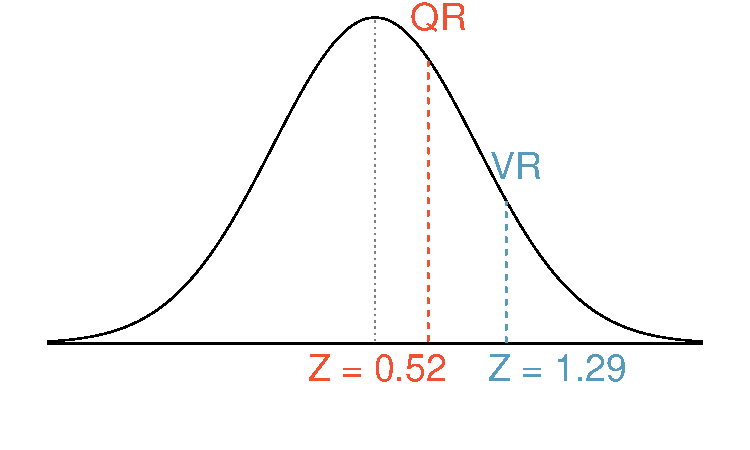
\includegraphics[width=0.3\textwidth]{ch_distributions/figures/eoce/gre/gre} \\
(c)~She scored 1.33 standard deviations above the mean on the Verbal Reasoning section and 0.57 standard deviations above the mean on the Quantitative Reasoning section.
(d)~She did better on the Verbal Reasoning section since her Z score on that section was higher.
(e)~$Perc_{VR} = 0.9082 \approx 91\%$, $Perc_{QR} = 0.7157 \approx 72\%$.
(f)~$100\% - 91\% = 9\%$ did better than her on VR, and $100\% - 72\% = 28\%$ did better than her on QR.
(g)~We cannot compare the raw scores since they are on different scales. Comparing her percentile scores is more appropriate when comparing her performance to others.
(h)~Answer to part (b) would not change as Z scores can be calculated for distributions that are not normal. However, we could not answer parts~(d)-(f) since we cannot use the normal probability table to calculate probabilities and percentiles without a normal model.}

% 5
\eocesol{(a)~$Z = 0.84$, which corresponds to 711 on QR.
(b)~$Z = -0.52$, which corresponds to 400 on VR.}

% 7
\eocesol{(a)~$Z=1.2 \to 0.1151$.
(b)~$Z= -1.28 \to 70.6\degree$F or colder.}

% 9
\eocesol{(a)~$N(25, 2.78)$.
(b)~$Z = 1.08 \to 0.1401$.
(c)~The answers are very close because only the units were changed. (The only reason why they are a little different is because 28\degree C is 82.4\degree F, not precisely 83\degree F.)}

% 11
\eocesol{(a)~$Z=0.67$.
(b)~$\mu=\$1650$, $x=\$1800$.
(c)~$0.67 = \frac{1800-1650}{\sigma} \to \sigma=\$223.88$.}

% 13
\eocesol{$Z = 1.56 \to 0.0594$, i.e. 6\%.}

% 15
\eocesol{(a)~$Z=0.73 \to 0.2327$.
(b)~If you are bidding on only one auction and set a low maximum bid price, someone will probably outbid you. If you set a high maximum bid price, you may win the auction but pay more than is necessary. If bidding on more than one auction, and you set your maximum bid price very low, you probably won't win any of the auctions. However, if the maximum bid price is even modestly high, you are likely to win multiple auctions.
(c)~An answer roughly equal to the 10th percentile would be reasonable. Regrettably, no percentile cutoff point guarantees beyond any possible event that you win at least one auction. However, you may pick a higher percentile if you want to be more sure of winning an auction.
(d)~Answers will vary a little but should correspond to the answer in part~(c). We use the 10$^{th}$ percentile: $Z = -1.28 \to \$69.80$.}

% 17
\eocesol{$14/20=70\%$ are within 1 SD. Within 2 SD: $19/20=95\%$. Within 3 SD: $20/20 = 100\%$. They follow this rule closely.}

% 19
\eocesol{The distribution is unimodal and symmetric. The superimposed normal curve approximates the distribution pretty well. The points on the normal probability plot also follow a relatively straight line. There is one slightly distant observation on the lower end, but it is not extreme. The data appear to be reasonably approximated by the normal distribution.}


% 21
\eocesol{(a)~The distribution is unimodal and strongly right skewed with a median between 5 and 10 years old. Ages range from 0 to slightly over 50 years old, and the middle 50\% of the distribution is roughly between 5 and 15 years old. There are potential outliers on the higher end.
(b)~When the sample size is small, the sampling distribution is right skewed, just like the population distribution. As the sample size increases, the sampling distribution gets more unimodal, symmetric, and approaches normality. The variability also decreases. This is consistent with the Central Limit Theorem.}

% 23
\eocesol{The centers are the same in each plot, and each data set is from a nearly normal distribution (see Section~\ref{nearlyNormalPopWithKnownSD}), though the histograms may not look very normal since each represents only 100 data points. The only way to tell which plot corresponds to which scenario is to examine the variability of each distribution. Plot B is the most variable, followed by Plot A, then Plot C. This means Plot B will correspond to the original data, Plot A to the sample means with size 5, and Plot C to the sample means with size 25.}

% 25
\eocesol{(a)~Right skewed. There is a long tail on the higher end of the distribution but a much shorter tail on the lower end.
(b)~Less than, as the median would be less than the mean in a right skewed distribution.
(c)~We should not.
(d)~Even though the population distribution is not normal, the conditions for inference are reasonably satisfied, with the possible exception of skew. If the skew isn't very strong (we should ask to see the data), then we can use the Central Limit Theorem to estimate this probability. For now, we'll assume the skew isn't very strong, though the description suggests it is at least moderate to strong. Use $N(1.3, SD_{\bar{x}} = 0.3/\sqrt{60})$: $Z=2.58$ $\to$ 0.0049.
(e)~It would decrease it by a factor of $1/\sqrt{2}$.}

% 27
\eocesol{(a)~$Z=-3.33$ $\to$ 0.0004.
(b)~The population SD is known and the data are nearly normal, so the sample mean will be nearly normal with distribution $N(\mu, \sigma/\sqrt{n})$, i.e. $N(2.5, 0.0095)$.
(c)~$Z=-10.54$ $\to$ $\approx0$.
(d)~See below:
\begin{center}
\includegraphics[width=0.48\textwidth]{ch_distributions/figures/eoce/penniesWeights/penniesWeights_sketch}
\end{center}
(e)~We could not estimate (a) without a nearly normal population distribution. We also could not estimate (c) since the sample size is not sufficient to yield a nearly normal sampling distribution if the population distribution is not nearly normal.}

% 29
\eocesol{(a)~We cannot use the normal model for this calculation, but we can use the histogram. About 500 songs are shown to be longer than 5 minutes, so the probability is about $500/3000 = 0.167$.
(b)~Two different answers are reasonable. $^{Option~1}$Since the population distribution is only slightly skewed to the right, even a small sample size will yield a nearly normal sampling distribution. We also know that the songs are sampled randomly and the sample size is less than 10\% of the population, so the length of one song in the sample is independent of another.  We are looking for the probability that the total length of 15 songs is more than 60 minutes, which means that the average song should last at least $60/15 = 4$ minutes. Using $SD_{\bar{x}}=1.63/\sqrt{15}$, $Z=1.31$ $\to$ 0.0951. $^{Option~2}$Since the population distribution is not normal, a small sample size may not be sufficient to yield a nearly normal sampling distribution. Therefore, we cannot estimate the probability using the tools we have learned so far.
(c)~We can now be confident that the conditions are satisfied. $Z = 0.92$ $\to$ 0.1788.}

% 31
\eocesol{(a)~$SD_{\bar{x}}=\frac{25}{\sqrt{75}}=2.89$.
(b)~$Z=1.73$, which indicates that the two values are not unusually distant from each other when accounting for the uncertainty in John's point estimate.}

%33
\eocesol{This is the same as checking that the average bag weight of the 10 bags is greater than 46 lbs. $SD_{\bar{x}}=\frac{3.2}{\sqrt{10}}=1.012$; $z= \frac{46-45}{1.012}=0.988$; $P(z > 0.988)=0.162=16.2\%$.}

% 35
\eocesol{(a) No. The cards are not independent. For example, if the first card is an ace of clubs, that implies the second card cannot be an ace of clubs. Additionally, there are many possible categories, which would need to be simplified.
(b) No. There are six events under consideration. The Bernoulli distribution allows for only two events or categories. Note that rolling a die could be a Bernoulli trial if we simply to two events, e.g. rolling a 6 and not rolling a 6, though specifying such details would be necessary.}

% 37
\eocesol{(a)~$(1-0.471)^2\times0.471 = 0.1318$.
(b)~$0.471^3 = 0.1045$.
(c)~$\mu = 1/0.471 = 2.12$, $\sigma=\sqrt{2.38} = 1.54$.
(d)~$\mu = 1/0.30 = 3.33$, $\sigma=2.79$.
(e)~When $p$ is smaller, the event is rarer, meaning the expected number of trials before a success and the standard deviation of the waiting time are higher.}

% 39
\eocesol{(a) $0.875^2\times 0.125 = 0.096$.
(b) $\mu=8$, $\sigma=7.48$.}

% 41
\eocesol{(a) $\mu=35$, $\sigma=3.24$.
(b) Yes. $Z=3.09$. Since 45 is more than 2 standard deviations from the mean, it would be considered unusual. Note that the normal model is not required to apply this rule of thumb.
(c) Using a normal model: 0.0010. This does indeed appear to be an unusual observation. If using a normal model with a 0.5 correction, the probability would be calculated as 0.0017.}



% 43
\eocesol{Want to find the probabiliy that there will be 1,786 or more enrollees. Using the normal: 0.0582. With a 0.5 correction: 0.0559.}

% 45
\eocesol{(a)~$1-0.75^3 = 0.5781$.
(b)~0.1406.
(c)~0.4219.
(d)~$1-0.25^3=0.9844$.}

% 47
\eocesol{(a)~Geometric distribution: 0.109.
(b)~Binomial: 0.219.
(c)~Binomial: 0.137.
(d)~$1-0.875^6=0.551$.
(e)~Geometric: 0.084.
(f)~Using a binomial distribution with $n = 6$ and $p=0.75$, we see that $\mu=4.5$, $\sigma=1.06$, and $Z = ?2.36$. Since this is not within 2 SD, it may be considered unusual.}

% 49
\eocesol{0 wins (-\$3): 0.1458. 1 win (-\$1): 0.3936. 2 wins (+\$1): 0.3543. 3 wins (+\$3): 0.1063.}



%51
\eocesol{(a)~Each observation in each of the distributions represents the sample proportion ($\hat{p}$) from samples of size  $n = 20$, $n = 100$, and $n = 500$, respectively. (b)~The centers for all three distributions are at 0.95, the true population parameter. When $n$ is small, the distribution is skewed to the left and not smooth. As $n$ increases, the variability of the distribution (standard deviation) decreases, and the shape of the distribution becomes more unimodal and symmetric.}

%53
\eocesol{(a)~The standard deviation of a sample proportion is given by $\sqrt{\frac{p(1-p)}{n}}=\sqrt{\frac{0.5(1-0.5)}{50}}=0.0707$. The average or expected variation in a sample of size 50 taken from this population is 0.0707. (b)~$Z=\frac{0.55-0.5}{0.0707}=0.707$; $P(Z > 0.707)=0.240$. }
\end{multicols}



\eocesolch{Foundation for inference}

\begin{multicols}{2}


% 1
\eocesol{(a)~Mean. Each student reports a numerical value: a number of hours.
(b)~Mean. Each student reports a number, which is a percentage, and we can average over these percentages.
(c)~Proportion. Each student reports Yes or No, so this is a categorical variable and we use a proportion.
(d)~Mean. Each student reports a number, which is a percentage like in part~(b).
(e)~Proportion. Each student reports whether or not s/he expects to get a job, so this is a categorical variable and we use a proportion.}

% 3
\eocesol{(a)~Mean: 13.65. Median: 14.
(b)~SD: 1.91. IQR: $15-13=2$.
(c)~$Z_{16}=1.23$, which is not unusual since it is within 2 SD of the mean. $Z_{18}=2.23$, which is generally considered unusual.
(d)~No. Point estimates that are based on samples only approximate the population parameter, and they vary from one sample to another.
(e)~We use the SE, which is $1.91/\sqrt{100}=0.191$ for this sample's mean.}

% 5
\eocesol{Recall that the general formula is
\begin{align*}
\text{point estimate} \pm z^{\star} \times SE
\end{align*}
First, identify the three different values. The point estimate is 45\%, $z^{\star} = 1.96$ for a 95\% confidence level, and $SE = 1.2\%$. Then, plug the values into the formula:
\begin{align*}
45\% \pm 1.96 \times 1.2\% \quad\to\quad (42.6\%, 47.4\%)
\end{align*}
We are 95\% confident that the proportion of US adults who live with one or more chronic conditions is between 42.6\% and 47.4\%.}

% 7
\eocesol{(a)~False. Confidence intervals provide a range of plausible values, and sometimes the truth is missed. A 95\% confidence interval ``misses'' about 5\% of the time.
(b)~True. Notice that the description focuses on the true population value.
(c)~True. If we examine the 95\% confidence interval computed in Exercise~\ref{ChronicIllnessP1}, we can see that 50\% is not included in this interval. This means that in a hypothesis test, we would reject the null hypothesis that the proportion is 0.5.
(d)~False. The standard error describes the uncertainty in the overall estimate from natural fluctuations due to randomness, not the uncertainty corresponding to individuals' responses.}

% 9
\eocesol{The subscript $_{pr}$ corresponds to provocative and $_{con}$ to conservative.
(a)~$H_0: p_{pr} = p_{con}$. $H_A: p_{pr} \ne p_{con}$.
(b)~-0.35.
(c)~The left tail for the p-value is calculated by adding up the two left bins: $0.005+0.015=0.02$. Doubling the one tail, the p-value is 0.04. (Students may have approximate results, and a small number of students may have a p-value of about 0.05.) Since the p-value is low, we reject $H_0$. The data provide strong evidence that people react differently under the two scenarios.}

%11
\eocesol{The primary concern is confirmation bias. If researchers look only for what they suspect to be true using a one-sided test, then they are formally excluding from consideration the possibility that the opposite result is true. Additionally, if other researchers believe the opposite possibility might be true, they would be very skeptical of the one-sided test.}

% 13
\eocesol{(a)~$H_0: p = 0.69$. $H_A: p \ne 0.69$.
(b)~$\hat{p} = \frac{17}{30} = 0.57$.
(c)~The success-failure condition is not satisfied; note that it is appropriate to use the null value ($p_0 = 0.69$) to compute the expected number of successes and failures.
(d)~Answers may vary. Each student can be represented with a card. Take 100 cards, 69 black cards representing those who follow the news about Egypt and 31 red cards representing those who do not. Shuffle the cards and draw with replacement (shuffling each time in between draws) 30 cards representing the 30 high school students. Calculate the proportion of black cards in this sample, $\hat{p}_{sim}$, i.e. the proportion of those who follow the news in the simulation. Repeat this many times (e.g. 10,000 times) and plot the resulting sample proportions. The p-value will be two times the proportion of simulations where $\hat{p}_{sim} \le 0.57$. (Note: we would generally use a computer to perform these simulations.)
(e)~The p-value is about $0.001 + 0.005 + 0.020 + 0.035 + 0.075 = 0.136$, meaning the two-sided p-value is about 0.272. Your p-value may vary slightly since it is based on a visual estimate. Since the p-value is greater than 0.05, we fail to reject $H_0$. The data do not provide strong evidence that the proportion of high school students who followed the news about Egypt is different than the proportion of American adults who did.}


\end{multicols}



\eocesolch{Inference for categorical data}

\begin{multicols}{2}

% 1
\eocesol{(a)~False. Doesn't satisfy success-failure condition.
(b)~True. The success-failure condition is not satisfied. In most samples we would expect $\hat{p}$ to be close to 0.08, the true population proportion. While $\hat{p}$ can be much above 0.08, it is bound below by 0, suggesting it would take on a right skewed shape. Plotting the sampling distribution would confirm this suspicion.
(c)~False. $SE_{\hat{p}} = 0.0243$, and $\hat{p} = 0.12$ is only $\frac{0.12 - 0.08}{0.0243} = 1.65$ SEs away from the mean, which would not be considered unusual.
(d)~True. $\hat{p}=0.12$ is 2.32 standard errors away from the mean, which is often considered unusual.
(e)~False. Decreases the SE by a factor of $1/\sqrt{2}$.}

% 3
\eocesol{(a)~True. See the reasoning of 6.1(b).
(b)~True. We take the square root of the sample size in the SE formula.
(c)~True. The independence and success-failure conditions are satisfied.
(d)~True. The independence and success-failure conditions are satisfied.}

% 5
\eocesol{(a)~False. A confidence interval is constructed to estimate the population proportion, not the sample proportion.
(b)~True. 95\% CI: $70\%\ \pm\ 8\%$.
(c)~True. By the definition of a confidence interval.
(d)~True. Quadrupling the sample size decreases the SE and ME by a factor of $1/\sqrt{4}$.
(e)~True. The 95\% CI is entirely above 50\%.}

% 7
\eocesol{With a random sample from $<10\%$ of the population, independence is satisfied. The success-failure condition is also satisfied. $ME = z^{\star} \sqrt{ \frac{\hat{p} (1-\hat{p})} {n} } = 1.96 \sqrt{ \frac{0.56 \times  0.44}{600} }= 0.0397 \approx 4\%$}

% 9
\eocesol{(a)~Proportion of graduates from this university who found a job within one year of graduating. $\hat{p} = 348/400 = 0.87$.
(b)~This is a random sample from less than 10\% of the population, so the observations are independent. Success-failure condition is satisfied: 348 successes, 52 failures, both well above~10.
(c)~(0.8371, 0.9029). We are 95\% confident that approximately 84\% to 90\% of graduates from this university found a job within one year of completing their undergraduate degree.
(d)~95\% of such random samples would produce a 95\% confidence interval that includes the true proportion of students at this university who found a job within one year of graduating from college.
(e)~(0.8267, 0.9133). Similar interpretation as before.
(f)~99\% CI is wider, as we are more confident that the true proportion is within the interval and so need to cover a wider range.}

% 11
\eocesol{(a)~No. The sample only represents students who took the SAT, and this was also an online survey.
(b)~(0.5289, 0.5711). We are 90\% confident that 53\% to 57\% of high school seniors who took the SAT are fairly certain that they will participate in a study abroad program in college.
(c)~90\% of such random samples would produce a 90\% confidence interval that includes the true proportion.
(d)~Yes. The interval lies entirely above 50\%.}

% 13
\eocesol{(a)~This is an appropriate setting for a hypothesis test. $H_0: p = 0.50$. $H_A:  p > 0.50$. Both independence and the success-failure condition are satisfied. $Z=1.12$ $\to$ p-value $= 0.1314$. Since the p-value $> \alpha=0.05$, we fail to reject $H_0$. The data do not provide strong evidence in favor of the claim.
(b)~Yes, since we did not reject $H_0$ in part~(a).}

% 15
\eocesol{(a)~$H_0: p = 0.38$. $H_A: p \ne 0.38$. Independence (random sample, $<10\%$ of population) and the success-failure condition are satisfied. $Z=-20.5$ $\to$ p-value $\approx 0$. Since the p-value is very small, we reject $H_0$. The data provide strong evidence that the proportion of Americans who only use their cell phones to access the internet is different than the Chinese proportion of 38\%, and the data indicate that the proportion is lower in the US.
(b)~If in fact 38\% of Americans used their cell phones as a primary access point to the internet, the probability of obtaining a random sample of 2,254 Americans where 17\% or less or 59\% or more use their only their cell phones to access the internet would be approximately 0.
(c)~(0.1545, 0.1855). We are 95\% confident that approximately 15.5\% to 18.6\% of all Americans primarily use their cell phones to browse the internet.}

% 17
\eocesol{(a)~$H_0: p = 0.5$. $H_A: p > 0.5$. Independence (random sample, $<10\%$ of population) is satisfied, as is the success-failure conditions (using $p_0 = 0.5$, we expect 40 successes and 40 failures). $Z = 2.91$ $\to$ p-value $= 0.0018$. Since the p-value $< 0.05$, we reject the null hypothesis. The data provide strong evidence that the rate of correctly identifying a soda for these people is significantly better than just by random guessing.
(b)~If in fact people cannot tell the difference between diet and regular soda and they randomly guess, the probability of getting a random sample of 80 people where 53 or more identify a soda correctly would be 0.0018.}

% 19
\eocesol{(a)~Independence is satisfied (random sample from $<10\%$ of the population), as is the success-failure condition (40 smokers, 160 non-smokers). The 95\% CI: (0.145, 0.255). We are 95\% confident that 14.5\% to 25.5\% of all students at this university smoke.
(b)~We want $z^{\star}SE$ to be no larger than 0.02 for a 95\% confidence level. We use $z^{\star}=1.96$ and plug in the point estimate $\hat{p}=0.2$ within the SE formula: $1.96\sqrt{0.2(1-0.2)/n} \leq 0.02$. The sample size $n$ should be at least 1,537.}

% 21
\eocesol{The margin of error, which is computed as $z^{\star}SE$, must be smaller than 0.01 for a 90\% confidence level. We use $z^{\star} = 1.65$ for a 90\% confidence level, and we can use the point estimate $\hat{p}=0.52$ in the formula for $SE$. $1.65\sqrt{0.52(1-0.52)/n} \leq 0.01$. Therefore, the sample size $n$ must be at least 6,796.}

% 23
\eocesol{This is not a randomized experiment, and it is unclear whether people would be affected by the behavior of their peers. That is, independence may not hold. Additionally, there are only 5 interventions under the provocative scenario, so the success-failure condition does not hold. Even if we consider a hypothesis test where we pool the proportions, the success-failure condition will not be satisfied. Since one condition is questionable and the other is not satisfied, the difference in sample proportions will not follow a nearly normal distribution.}

% 25
\eocesol{(a)~False. The entire confidence interval is above 0.
(b)~True.
(c)~True.
(d)~True.
(e)~False. It is simply the negated and reordered values: (-0.06,-0.02).}

% 27
\eocesol{(a)~(0.23, 0.33). We are 95\% confident that the proportion of Democrats who support the plan is 23\% to 33\% higher than the proportion of Independents who do.
(b)~True.}

% 29
\eocesol{(a)~College grads: 23.7\%. Non-college grads: 33.7\%.
(b)~Let $p_{CG}$ and $p_{NCG}$ represent the proportion of college graduates and non-college graduates who responded ``do not know". $H_0: p_{CG} = p_{NCG}$. $H_A: p_{CG} \ne p_{NCG}$. Independence is satisfied (random sample, $<10\%$ of the population), and the success-failure condition, which we would check using the pooled proportion ($\hat{p} = 235/827 = 0.284$), is also satisfied. $Z=-3.18$ $\to$ p-value = 0.0014. Since the p-value is very small, we reject $H_0$. The data provide strong evidence that the proportion of college graduates who do not have an opinion on this issue is different than that of non-college graduates. The data also indicate that fewer college grads say they ``do not know'' than non-college grads (i.e. the data indicate the direction after we reject $H_0$).}

% 31
\eocesol{(a)~College grads: 35.2\%. Non-college grads: 33.9\%.
(b)~Let $p_{CG}$ and $p_{NCG}$ represent the proportion of college graduates and non-college grads who support offshore drilling. $H_0: p_{CG} = p_{NCG}$. $H_A: p_{CG} \ne p_{NCG}$. Independence is satisfied (random sample, $<10\%$ of the population), and the success-failure condition, which we would check using the pooled proportion ($\hat{p} = 286/827 = 0.346$), is also satisfied. $Z = 0.39$ $\to$ p-value $=0.6966$. Since the p-value $> \alpha$ (0.05), we fail to reject $H_0$. The data do not provide strong evidence of a difference between the proportions of college graduates and non-college graduates who support off-shore drilling in California.}

% 33
\eocesol{Subscript $_C$ means control group. Subscript $_T$ means truck drivers.
(a)~$H_0: p_C = p_T$. $H_A: p _C \ne p_T$. Independence is satisfied (random samples, $<10\%$ of the population), as is the success-failure condition, which we would check using the pooled proportion ($\hat{p} = 70/495 = 0.141$). $Z = -1.58$ $\to$ p-value $=0.1164$. Since the p-value is high, we fail to reject $H_0$. The data do not provide strong evidence that the rates of sleep deprivation are different for non-transportation workers and truck drivers.}

% 35
\eocesol{(a)~Summary of the study:
\begin{center}\scriptsize
\begin{tabular}{l l c c c}
								&			& \multicolumn{2}{c}{\textit{Virol. failure}}	&		\\
\cline{3-4}
								&			& Yes		& No		& Total	\\
\cline{2-5}
\multirow{2}{*}{\textit{Treatment}}		& Nevaripine	& 26			& 94		& 120	\\
								& Lopinavir	& 10			& 110	& 120	\\
\cline{2-5}
								& Total		& 36			& 204	& 240
\end{tabular}
\end{center}
(b)~$H_0: p_N = p_L$. There is no difference in virologic failure rates between the Nevaripine and Lopinavir groups. $H_A: p_N \ne p_L$. There is some difference in virologic failure rates between the Nevaripine and Lopinavir groups.
(c)~Random assignment was used, so the observations in each group are independent. If the patients in the study are representative of those in the general population (something impossible to check with the given information), then we can also confidently generalize the findings to the population. The success-failure condition, which we would check using the pooled proportion ($\hat{p} = 36/240 = 0.15$), is satisfied. $Z=3.04$ $\to$ p-value $=0.0024$. Since the p-value is low, we reject $H_0$. There is strong evidence of a difference in virologic failure rates between the Nevaripine and Lopinavir groups do not appear to be independent.}

% 37
\eocesol{(a)~False. The chi-square distribution has one parameter called degrees of freedom.
(b)~True.
(c)~True.
(d)~False. As the degrees of freedom increases, the shape of the chi-square distribution becomes more symmetric.}

% 39
\eocesol{(a)~$H_0$: The distribution of the format of the book used by the students follows the professor's predictions. $H_A$: The distribution of the format of the book used by the students does not follow the professor's predictions.
(b)~$E_{hard~copy} = 126 \times  0.60 = 75.6$. $E_{print} = 126 \times  0.25 = 31.5$. $E_{online} = 126 \times  0.15 = 18.9$.
(c)~Independence:  The sample is not random. However, if the professor has reason to believe that the proportions are stable from one term to the next and students are not affecting each other's study habits, independence is probably reasonable. Sample size: All expected counts are at least 5. Degrees of freedom: $df = k - 1 = 3 - 1 = 2$ is more than 1.
(d)~$X^2 = 2.32$, $df=2$, p-value $> 0.3$.
(e)~Since the p-value is large, we fail to reject $H_0$. The data do not provide strong evidence indicating the professor's predictions were statistically inaccurate.}

% 41
\eocesol{(a). Two-way table:
\begin{center}\scriptsize
\begin{tabular}{l l c c c}
& \multicolumn{2}{c}{\textit{Quit}}	&		\\
\cline{2-3}
\textit{Treatment}		& Yes		& No		& Total	\\
\hline
Patch + support group	& 40			& 110	& 150	\\
Only patch			& 30			& 120	& 150	\\
\cline{1-4}
Total				& 70			& 230	& 300 \\
\cline{1-4}
\end{tabular}
\end{center}
(b-i)~$E_{row_1, col_1} = \frac{(row~1~total)\times(col~1~total)}{table~total} = \frac{150 \times  70}{300} = 35$. This is lower than the observed value.
(b-ii)~$E_{row_2, col_2} = \frac{(row~2~total)\times(col~2~total)}{table~total} = \frac{150 \times  230}{300} = 115$. This is lower than the observed value.}

% 43
\eocesol{$H_0$: The opinion of college grads and non-grads is not different on the topic of drilling for oil and natural gas off the coast of California. $H_A$: Opinions regarding the drilling for oil and natural gas off the coast of California has an association with earning a college degree.
\begin{align*}
&E_{row~1, col~1} = 151.5 && E_{row~1, col~2} = 134.5 \\
&E_{row~2, col~1} = 162.1 && E_{row~2, col~2} = 143.9 \\
&E_{row~3, col~1} = 124.5 && E_{row~3, col~2} = 110.5
\end{align*}
Independence: The samples are both random, unrelated, and from less than 10\% of the population, so independence between observations is reasonable. Sample size: All expected counts are at least 5. Degrees of freedom: $df = (R - 1) \times  (C - 1) = (3 - 1) \times  (2 - 1) = 2$, which is greater than 1.
$X^2 = 11.47$, $df = 2$ $\to$ $0.001<$ p-value $<0.005$.
Since the p-value $< \alpha$, we reject $H_0$.  There is strong evidence that there is an association between support for off-shore drilling and having a college degree.}

% 45
\eocesol{(a)~$H_0$:~The age of Los Angeles residents is independent of shipping carrier preference variable. $H_A$:~The age of Los Angeles residents is associated with the shipping carrier preference variable. (b)~The conditions are not satisfied since some expected counts are below~5.}

%% 45
%\eocesol{(a)~$H_0:$ There is no relationship between gender and how informed Facebook users are about adjusting their privacy settings. $H_A:$ There is a relationship between gender and how informed Facebook users are about adjusting their privacy settings.
%(b)~The expected counts:
%\begin{align*}
%&E_{row~1,col~1} = 296.6 && E_{row~1,col~2} = 369.3 \\
%&E_{row~2,col~1} = 54.8 && E_{row~2,col~2} = 68.2 \\
%&E_{row~3,col~1} = 7.6 && E_{row~3,col~2} = 9.4
%\end{align*}
%The sample is random, all expected counts are above 5, and $df=(3-1)\times(2-1) = 2 > 1$, so we may proceed with the test.} %%%%The test statistic may be computed as $X^2 = 3.1291$ with $df= 2$. The p-value is greater than 0.2, indicating that the evidence is not sufficiently strong for us to reject the null hypothesis. That is, the data do not provide sufficiently strong evidence to conclude that Facebook users knowledge about privacy settings varies by gender.}


\end{multicols}





\eocesolch{Inference for numerical data}

\begin{multicols}{2}


\textB{\pagebreak}

% 1
\eocesol{(a)~$df=6-1=5$, $t_{5}^{\star} = 2.02$ (column with two tails of 0.10, row with $df=5$).
(b)~$df=21-1=20$, $t_{20}^{\star} = 2.53$ (column with two tails of 0.02, row with $df=20$).
(c)~$df=28$, $t_{28}^{\star} = 2.05$.
(d)~$df=11$, $t_{11}^{\star} = 3.11$.}

% 3
\eocesol{The mean is the midpoint: $\bar{x} = 20$. Identify the margin of error: $ME = 1.015$, then use $t^{\star}_{35} = 2.03$ and $SE=s/\sqrt{n}$ in the formula for margin of error to identify $s = 3$.}

% 5
\eocesol{(a)~$H_0$: $\mu = 8$ (New Yorkers sleep 8 hrs per night on average.) $H_A$: $\mu < 8$ (New Yorkers sleep less than 8 hrs per night on average.)
(b)~Independence: The sample is random and from less than 10\% of New Yorkers. The sample is small, so we will use a $t$ distribution. For this size sample, slight skew is acceptable, and the min/max suggest there is not much skew in the data. $T = -1.75$. $df=25-1=24$.
(c)~$0.025 <$ p-value $<0.05$. If in fact the true population mean of the amount New Yorkers sleep per night was 8 hours, the probability of getting a random sample of 25 New Yorkers where the average amount of sleep is 7.73 hrs per night or less is between 0.025 and 0.05.
(d)~Since p-value $<$ 0.05, reject $H_0$. The data provide strong evidence that New Yorkers sleep less than 8 hours per night on average.
(e)~No, as we rejected $H_0$.}

% 7
\eocesol{$t^{\star}_{19}$ is 1.73 for a one-tail. We want the lower tail, so set -1.73 equal to the T score, then solve for $\bar{x}$: 56.91.}

% 9
\eocesol{(a)~For each observation in one data set, there is exactly one specially-corresponding observation in the other data set for the same geographic location. The data are paired.
(b)~$H_0: \mu_{diff} = 0$ (There is no difference in average daily high temperature between January 1, 1968 and January 1, 2008 in the continental US.) $H_A: \mu_{diff} > 0$ (Average daily high temperature in January 1, 1968 was lower than average daily high temperature in January, 2008 in the continental US.) If you chose a two-sided test, that would also be acceptable. If this is the case, note that your p-value will be a little bigger than what is reported here in part~(d).
(c)~Independence: locations are random and represent less than 10\% of all possible locations in the US. The sample size is at least 30. We are not given the distribution to check the skew. In practice, we would ask to see the data to check this condition, but here we will move forward under the assumption that it is not strongly skewed.
(d)~$Z=1.60$ $\to$ p-value $=0.0548$.
(e)~Since the p-value $> \alpha$ (since not given use 0.05), fail to reject $H_0$. The data do not provide strong evidence of temperature warming in the continental US. However it should be noted that the p-value is very close to 0.05.
(f)~Type 2, since we may have incorrectly failed to reject $H_0$. There may be an increase, but we were unable to detect it.
(g)~Yes, since we failed to reject $H_0$, which had a null value of 0.}

% 11
\eocesol{(a)~(-0.03, 2.23).
(b)~We are 90\% confident that the average daily high on January 1, 2008 in the continental US was 0.03 degrees lower to 2.23 degrees higher than the average daily high on January 1, 1968.
(c)~No, since 0 is included in the interval.}

% 13
\eocesol{(a)~Each of the 36 mothers is related to exactly one of the 36 fathers (and vice-versa), so there is a special correspondence between the mothers and fathers.
(b)~$H_0: \mu_{diff} = 0$. $H_A: \mu_{diff} \ne 0$. Independence: random sample from less than 10\% of population. Sample size of at least 30. The skew of the differences is, at worst, slight. $Z = 2.72$ $\to$ p-value $= 0.0066$. Since p-value $<$ 0.05, reject $H_0$. The data provide strong evidence that the average IQ scores of mothers and fathers of gifted children are different, and the data indicate that mothers' scores are higher than fathers' scores for the parents of gifted children.}


% 15
\eocesol{No, he should not move forward with the test since the distributions of total personal income are very strongly skewed. When sample sizes are large, we can be a bit lenient with skew. However, such strong skew observed in this exercise would require somewhat large sample sizes, somewhat higher than~30.}

% 17
\eocesol{(a)~These data are paired. For example, the Friday the 13th in say, September 1991, would probably be more similar to the Friday the 6th in September 1991 than to Friday the 6th in another month or year.
(b)~Let $\mu_{diff} = \mu_{sixth} - \mu_{thirteenth}$. $H_0: \mu_{diff} = 0$. $H_A: \mu_{diff} \ne 0$.
(c)~Independence: The months selected are not random. However, if we think these dates are roughly equivalent to a simple random sample of all such Friday 6th/13th date pairs, then independence is reasonable. To proceed, we must make this strong assumption, though we should note this assumption in any reported results. With fewer than 10 observations, we would need to use the $t$ distribution to model the sample mean. The normal probability plot of the differences shows an approximately straight line. There isn't a clear reason why this distribution would be skewed, and since the normal quantile plot looks reasonable, we can mark this condition as reasonably satisfied.
(d)~$T = 4.94$ for $df=10-1=9$ $\to$ p-value $<0.01$.
(e)~Since p-value $<$ 0.05, reject $H_0$. The data provide strong evidence that the average number of cars at the intersection is higher on Friday the 6$^{\text{th}}$ than on Friday the 13$^{\text{th}}$. (We might believe this intersection is representative of all roads, i.e. there is higher traffic on Friday the 6$^{\text{th}}$ relative to Friday the 13$^{\text{th}}$. However, we should be cautious of the required assumption for such a generalization.)
(f)~If the average number of cars passing the intersection actually was the same on Friday the 6$^{\text{th}}$ and $13^{th}$, then the probability that we would observe a test statistic so far from zero is less than 0.01.
(g)~We might have made a Type 1 error, i.e. incorrectly rejected the null hypothesis.}

% 19
\eocesol{(a)~$H_0: \mu_{diff} = 0$. $H_A: \mu_{diff} \ne 0$. $T=-2.71$. $df=5$. $0.02<$ p-value $<0.05$. Since p-value $<$ 0.05, reject $H_0$. The data provide strong evidence that the average number of traffic accident related emergency room admissions are different between Friday the 6$^{\text{th}}$ and Friday the 13$^{\text{th}}$. Furthermore, the data indicate that the direction of that difference is that accidents are lower on Friday the $6^{th}$ relative to Friday the 13$^{\text{th}}$.
(b)~(-6.49, -0.17).
(c)~This is an observational study, not an experiment, so we cannot so easily infer a causal intervention implied by this statement. It is true that there is a difference. However, for example, this does not mean that a responsible adult going out on Friday the $13^{th}$ has a higher chance of harm than on any other night.}

% 21
\eocesol{(a)~Chicken fed linseed weighed an average of 218.75 grams while those fed horsebean weighed an average of 160.20 grams. Both distributions are relatively symmetric with no apparent outliers. There is more variability in the weights of chicken fed linseed.
(b)~$H_0: \mu_{ls} = \mu_{hb}$. $H_A: \mu_{ls} \ne \mu_{hb}$. We leave the conditions to you to consider. $T=3.02$, $df = min(11, 9) = 9$ $\to$ $0.01<$ p-value $<0.02$. Since p-value $<$ 0.05, reject $H_0$. The data provide strong evidence that there is a significant difference between the average weights of chickens that were fed linseed and horsebean.
(c)~Type 1, since we rejected $H_0$.
(d)~Yes, since p-value $>$ 0.01, we would have failed to reject~$H_0$.}

% 23
\eocesol{$H_0: \mu_C = \mu_S$. $H_A: \mu_C \ne \mu_S$. $T = 3.27$, $df=11$ $\to$ p-value $<0.01$. Since p-value $< 0.05$, reject $H_0$. The data provide strong evidence that the average weight of chickens that were fed casein is different than the average weight of chickens that were fed soybean (with weights from casein being higher). Since this is a randomized experiment, the observed difference can be attributed to the diet.}

% 25
\eocesol{$H_0: \mu_{T} = \mu_{C}$. $H_A: \mu_{T} \ne \mu_{C}$. $T=2.24$, $df=21$ $\to$ $0.02<$ p-value $<0.05$. Since p-value $<$ 0.05, reject $H_0$. The data provide strong evidence that the average food consumption by the patients in the treatment and control groups are different. Furthermore, the data indicate patients in the distracted eating (treatment) group consume more food than patients in the control group.}

% 27
\eocesol{Let $\mu_{diff} = \mu_{pre} - \mu_{post}$. $H_0: \mu_{diff} = 0$: Treatment has no effect. $H_A: \mu_{diff} > 0$: Treatment is effective in reducing Pd T scores, the average pre-treatment score is higher than the average post-treatment score. Note that the reported values are pre minus post, so we are looking for a positive difference, which would correspond to a reduction in the psychopathic deviant T score. Conditions are checked as follows. Independence: The subjects are randomly assigned to treatments, so the patients in each group are independent. All three sample sizes are smaller than 30, so we use $t$ tests.Distributions of differences are somewhat skewed. The sample sizes are small, so we cannot reliably relax this assumption. (We will proceed, but we would not report the results of this specific analysis, at least for treatment group 1.) For all three groups: $df=13$. $T_1= 1.89$ ($0.025<$ p-value $<0.05$), $T_2=1.35$ (p-value = 0.10), $T_3 = -1.40$ (p-value $>0.10$). The only significant test reduction is found in Treatment 1, however, we had earlier noted that this result might not be reliable due to the skew in the distribution. Note that the calculation of the p-value for Treatment 3 was unnecessary: the sample mean indicated a increase in Pd T scores under this treatment (as opposed to a decrease, which was the result of interest). That is, we could tell without formally completing the hypothesis test that the p-value would be large for this treatment group.}

% 29
\eocesol{$H_0$: $\mu_1 = \mu_2 = \cdots = \mu_6$. $H_A$: The average weight varies across some (or all) groups. Independence: Chicks are randomly assigned to feed types (presumably kept separate from one another), therefore independence of observations is reasonable. Approx. normal: the distributions of weights within each feed type appear to be fairly symmetric. Constant variance: Based on the side-by-side box plots, the constant variance assumption appears to be reasonable. There are differences in the actual computed standard deviations, but these might be due to chance as these are quite small samples. $F_{5,65} = 15.36$ and the p-value is approximately 0. With such a small p-value, we reject $H_0$. The data provide convincing evidence that the average weight of chicks varies across some (or all) feed supplement groups.}

%\end{multicols}

% 31
\eocesol{(a)~$H_0$: The population mean of MET for each group is equal to the others. $H_A$: At least one pair of means is different.
(b)~Independence: We don't have any information on how the data were collected, so we cannot assess independence. To proceed, we must assume the subjects in each group are independent. In practice, we would inquire for more details. Approx. normal: The data are bound below by zero and the standard deviations are larger than the means, indicating very strong strong skew. However, since the sample sizes are extremely large, even extreme skew is acceptable. Constant variance: This condition is sufficiently met, as the standard deviations are reasonably consistent across groups.
(c)~See below, with the last column omitted:\\[-2mm]
\begin{adjustwidth}{-4em}{-4em}
{\tiny
\begin{center}
\renewcommand{\arraystretch}{1.25}
\begin{tabular}{lrrrr}
  \hline
 			& Df 	& Sum Sq		& Mean Sq	& F value \\ 
  \hline
coffee	 	& {\textcolor{oiB}{{\scriptsize 4}}}	 & {\textcolor{oiB}{{\scriptsize 10508}}} 		& {\textcolor{oiB}{{\scriptsize 2627}}} 			& {\textcolor{oiB}{{\scriptsize 5.2}}} \\ 
Residuals		& {\textcolor{oiB}{{\scriptsize 50734}}} & 25564819 	& {\textcolor{oiB}{{\scriptsize  504}}} 		&  \\ 
   \hline
Total			& {\textcolor{oiB}{{\scriptsize 50738}}} & 25575327 \\
\hline
\end{tabular}
\end{center}
}
\end{adjustwidth} \vspace{1mm}
(d)~Since p-value is very small, reject $H_0$. The data provide convincing evidence that the average MET differs between at least one pair of groups.}

%\begin{multicols}{2}

% 33
\eocesol{(a)~$H_0$: Average GPA is the same for all majors. $H_A$: At least one pair of means are different.
(b)~Since p-value $>$ 0.05, fail to reject $H_0$. The data do not provide convincing evidence of a difference between the average GPAs across three groups of majors.
(c)~The total degrees of freedom is $195 + 2 = 197$, so the sample size is $197+1=198$.}

% 35
\eocesol{(a)~False. As the number of groups increases, so does the number of comparisons and hence the modified significance level decreases.
(b)~True.
(c)~True.
(d)~False. We need observations to be independent regardless of sample size.}

% 37
\eocesol{(a)~$H_0$: Average score difference is the same for all treatments. $H_A$: At least one pair of means are different.
(b)~We should check conditions. If we look back to the earlier exercise, we will see that the patients were randomized, so independence is satisfied. There are some minor concerns about skew, especially with the third group, though this may be acceptable. The standard deviations across the groups are reasonably similar. Since the p-value is less than 0.05, reject $H_0$. The data provide convincing evidence of a difference between the average reduction in score among treatments.
(c)~We determined that at least two means are different in part (b), so we now conduct $K=3\times2/2=3$ pairwise $t$ tests that each use $\alpha=0.05/3 = 0.0167$ for a significance level. Use the following hypotheses for each pairwise test. $H_0$: The two means are equal. $H_A$: The two means are different. The sample sizes are equal and we use the pooled SD, so we can compute $SE=3.7$ with the pooled $df=39$. The p-value only for Trmt 1 vs. Trmt 3 may be statistically significant: $0.01<$ p-value $<0.02$. Since we cannot tell, we should use a computer to get the p-value, 0.015, which is statistically significant for the adjusted significance level. That is, we have identified Treatment 1 and Treatment 3 as having different effects. Checking the other two comparisons, the differences are not statistically significant.}

\end{multicols}
















%\textB{\pagebreak}

\eocesolch{Introduction to linear regression}

\begin{multicols}{2}

% 1
\eocesol{(a)~The residual plot will show randomly distributed residuals around 0. The variance is also approximately constant.
(b)~The residuals will show a fan shape, with higher variability for smaller $x$. There will also be many points on the right above the line. There is trouble with the model being fit here.}

% 3
\eocesol{(a)~Strong relationship, but a straight line would not fit the data.
(b)~Strong relationship, and a linear fit would be reasonable.
(c)~Weak relationship, and trying a linear fit would be reasonable.
(d)~Moderate relationship, but a straight line would not fit the data. (e)~Strong relationship, and a linear fit would be reasonable.
(f)~Weak relationship, and trying a linear fit would be reasonable.}

% 5
\eocesol{(a)~Exam 2 since there is less of a scatter in the plot of final exam grade versus exam 2. Notice that the relationship between Exam 1 and the Final Exam appears to be slightly nonlinear.
(b)~Exam 2 and the final are relatively close to each other chronologically, or Exam 2 may be cumulative so has greater similarities in material to the final exam. Answers may vary for part~(b).}

% 7
\eocesol{(a)~$R = -0.7$ $\rightarrow$ (4).
(b)~$R = 0.45$  $\rightarrow$ (3).
(c)~$R = 0.06$ $\rightarrow$ (1).
(d)~$R = 0.92$ $\rightarrow$ (2).}

% 9
\eocesol{(a)~The relationship is positive, weak, and possibly linear. However, there do appear to be some anomalous observations along the left where several students have the same height that is notably far from the cloud of the other points. Additionally, there are many students who appear not to have driven a car, and they are represented by a set of points along the bottom of the scatterplot.
(b)~There is no obvious explanation why simply being tall should lead a person to drive faster. However, one confounding factor is gender. Males tend to be taller than females on average, and personal experiences (anecdotal) may suggest they drive faster. If we were to follow-up on this suspicion, we would find that sociological studies confirm this suspicion.
(c)~Males are taller on average and they drive faster. The gender variable is indeed an important confounding variable.}

% 11
\eocesol{(a)~There is a somewhat weak, positive, possibly linear relationship between the distance traveled and travel time. There is clustering near the lower left corner that we should take special note of.
(b)~Changing the units will not change the form, direction or strength of the relationship between the two variables. If longer distances measured in miles are associated with longer travel time measured in minutes, longer distances measured in kilometers will be associated with longer travel time measured in hours.
(c)~Changing units doesn't affect correlation: $R = 0.636$.}

% 13

\eocesol{(a)~There is a moderate, positive, and linear relationship between shoulder girth and height.
(b)~Changing the units, even if just for one of the variables, will not change the form, direction or strength of the relationship between the two variables.}

% 15

\eocesol{In each part, we may write the husband ages as a linear function of the wife ages: (a) $age_{H} = age_{W} + 3$; (b) $age_{H} = age_{W} - 2$; and (c) $age_{H} = 2 \times age_{W}$. Therefore, the correlation will be exactly 1 in all three parts. An alternative way to gain insight into this solution is to create a mock data set, such as a data set of 5 women with ages 26, 27, 28, 29, and 30 (or some other set of ages). Then, based on the description, say for part (a), we can compute their husbands' ages as 29, 30, 31, 32, and 33. We can plot these points to see they fall on a straight line, and they always will. The same approach can be applied to the other parts as well.}

% 17

\eocesol{(a)~There is a positive, very strong, linear association between the number of tourists and spending.
(b)~Explanatory: number of tourists (in thousands). Response: spending (in millions of US dollars).
(c)~We can predict spending for a given number of tourists using a regression line. This may be useful information for determining how much the country may want to spend in advertising abroad, or to forecast expected revenues from tourism.
(d)~Even though the relationship appears linear in the scatterplot, the residual plot actually shows a nonlinear relationship. This is not a contradiction: residual plots can show divergences from linearity that can be difficult to see in a scatterplot. A simple linear model is inadequate for modeling these data. It is also important to consider that these data are observed sequentially, which means there may be a hidden structure that it is not evident in the current data but that is important to consider.}

% 19

\eocesol{(a)~First calculate the slope: $b_1 = R\times s_y/s_x = 0.636\times113/99 = 0.726$. Next, make use of the fact that the regression line passes through the point $(\bar{x},\bar{y})$: $\bar{y} = b_0 + b_1 \times \bar{x}$. Plug in $\bar{x}$, $\bar{y}$, and $b_1$, and solve for $b_0$: 51. Solution: $\widehat{travel~time} = 51 + 0.726 \times distance$.
(b)~$b_1$: For each additional mile in distance, the model predicts an additional 0.726 minutes in travel time. $b_0$: When the distance traveled is 0 miles, the travel time is expected to be 51 minutes. It does not make sense to have a travel distance of 0 miles in this context. Here, the $y$-intercept serves only to adjust the height of the line and is meaningless by itself.
(c)~$R^2 = 0.636^2 = 0.40$. About 40\% of the variability in travel time is accounted for by the model, i.e. explained by the distance traveled.
(d)~$\widehat{travel~time} =  51 + 0.726 \times distance = 51 + 0.726 \times 103 \approx 126$ minutes. (Note: we should be cautious in our predictions with this model since we have not yet evaluated whether it is a well-fit model.)
(e)~$e_i = y_i - \hat{y}_i = 168 - 126 = 42$ minutes. A positive residual means that the model underestimates the travel time.
(f)~No, this calculation would require extrapolation.}

% 21

\eocesol{(a)~$\sqrt{R^2} = 0.849$. Since the trend is negative, $R$ is also negative: $R=-0.849$.
(b)~$b_0 = 55.34$. $b_1 = -0.537$.
(c)~For a neighborhood with 0\% reduced-fee lunch, we would expect 55.34\% of the bike riders to wear helmets.
(d)~For every additional percentage point of reduced fee lunches in a neighborhood, we would expect 0.537\% fewer kids to be wearing helmets. %For every additional percentage point of lunch, there is a decrease of 0.537 percentage points in helmet.
(e)~$\hat{y} = 40\times(-0.537)+55.34 = 33.86$, $e = 40 - \hat y = 6.14$. There are 6.14\% more bike riders wearing helmets than predicted by the regression model in this neighborhood.}

% 23

\eocesol{(a)~The outlier is in the upper-left corner. Since it is horizontally far from the center of the data, it is a point with high leverage. Since the slope of the regression line would be very different if fit without this point, it is also an influential point.
(b)~The outlier is located in the lower-left corner. It is horizontally far from the rest of the data, so it is a high-leverage point. The line again would look notably different if the fit excluded this point, meaning it the outlier is influential.
(c)~The outlier is in the upper-middle of the plot. Since it is near the horizontal center of the data, it is not a high-leverage point. This means it also will have little or no influence on the slope of the regression line.}

% 25

\eocesol{(a)~There is a negative, moderate-to-strong, somewhat linear relationship between percent of families who own their home and the percent of the population living in urban areas in 2010. There is one outlier: a state where 100\% of the population is urban. The variability in the percent of homeownership also increases as we move from left to right in the plot.
(b)~The outlier is located in the bottom right corner, horizontally far from the center of the other points, so it is a point with high leverage. It is an influential point since excluding this point from the analysis would greatly affect the slope of the regression line.}

% 27

\eocesol{The relationship between the variables is somewhat linear. However, there are two apparent outliers. The residuals do not show a random scatter around 0. A simple linear model may not be appropriate for these data, and we should investigate the two outliers.}

% 29

\eocesol{(a)~The relationship is positive, moderate-to-strong, and linear. There are a few outliers but no points that appear to be influential.
(b)~$\widehat{weight} = -105.0113 + 1.0176 \times height$. Slope: For each additional centimeter in height, the model predicts the average weight to be 1.0176 additional kilograms (about 2.2 pounds).  Intercept: People who are 0 centimeters tall are expected to weigh -105.0113 kilograms. This is obviously not possible. Here, the $y$-intercept serves only to adjust the height of the line and is meaningless by itself.
(c)~$H_0$: The true slope coefficient of height is zero ($\beta_1 = 0$). $H_0$: The true slope coefficient of height is greater than zero ($\beta_1 > 0$). A two-sided test would also be acceptable for this application. The p-value for the two-sided alternative hypothesis ($\beta_1 \ne 0$) is incredibly small, so the p-value for the one-sided hypothesis will be even smaller. That is, we reject $H_0$. The data provide convincing evidence that height and weight are positively correlated. The true slope parameter is indeed greater than~0.
(d)~$R^2 = 0.72^2 = 0.52$. Approximately 52\% of the variability in weight can be explained by the height of individuals.}

% 31

\eocesol{(a)~$H_0$: $\beta_1 = 0$. $H_A$: $\beta_1 > 0$. A two-sided test would also be acceptable for this application. The p-value, as reported in the table, is incredibly small. Thus, for a one-sided test, the p-value will also be incredibly small, and we reject $H_0$. The data provide convincing evidence that wives' and husbands' heights are positively correlated. %However, whether this information is practically significant is unclear.
(b)~$\widehat{height}_{W} = 43.5755 + 0.2863 \times height_{H}$.
(c)~Slope: For each additional inch in husband's height, the average wife's height is expected to be an additional 0.2863 inches on average. Intercept: Men who are 0 inches tall are expected to have wives who are, on average, 43.5755 inches tall. The intercept here is meaningless, and it serves only to adjust the height of the line.
(d)~The slope is positive, so $R$ must also be positive. $R = \sqrt{0.09} = 0.30$.
(e)~63.2612. Since $R^2$ is low, the prediction based on this regression model is not very reliable.
(f)~No, we should avoid extrapolating.}

% 33

\eocesol{(a)~25.75.
(b)~$H_0$: $\beta_1 = 0$. $H_A$: $\beta_1 \ne 0$. A one-sided test also may be reasonable for this application. $T=2.23$, $df=23$ $\to$ p-value between 0.02 and 0.05. So we reject $H_0$. There is an association between gestational age and head circumference. We can also say that the association is positive.}

\end{multicols}


